\documentclass[a4paper,12pt]{article}
\usepackage[english]{babel}
\usepackage[utf8]{inputenc}
\usepackage{fontspec}
\setmainfont{CMU Serif}

\newfontfamily{\englishfont}{CMU Serif}
\newfontfamily{\thaifont}[Scale=MatchUppercase]{TH Sarabun Chula}
\newenvironment{thailang}{\thaifont}

\usepackage[Latin,Thai]{ucharclasses}
\setTransitionTo{Thai}{\thaifont}
\setTransitionFrom{Thai}{\englishfont}

\XeTeXlinebreaklocale "th_TH"
\XeTeXlinebreakskip = 0pt plus 1pt 

\usepackage{setspace}
\onehalfspacing

\usepackage{amsmath,amsthm,amssymb}
\usepackage{physics}
\usepackage{siunitx}
\usepackage[margin=1in]{geometry}
\usepackage{graphicx}
\usepackage{hyperref}

\renewcommand{\thefootnote}{\fnsymbol{footnote}}
	
\title{พาราโบลาปลอดภัย (Parabola of Safety)}
\author{อิธิพัฒน์ ธนบดีกาญจน์}

\begin{document}
	
\maketitle

\section{บทนำ}
ในวิชาฟิสิกส์ พาราโบลาปลอดภัย คือ พาราโบลาที่บ่งบอกถึงขอบเขตของโพรเจกไทล์\footnote{วัตถุใด ๆ ที่ถูกขว้างหรือถูกยิงออกไป}ที่จะสามารถเคลื่อนที่ไปได้ ซึ่งจะมีประโยชน์มากต่อการคำนวณโจทย์โพรเจกไทล์ที่ซับซ้อนโดยจะนำไปใช้ใน ปริภูมิ 2 มิติ หรือ ปริภูมิ 3 มิติ และถ้าวาดกราฟในปริภูมิ 3 มิติ จะได้รูปดังนี้
	\begin{figure}[h]
		\centering
		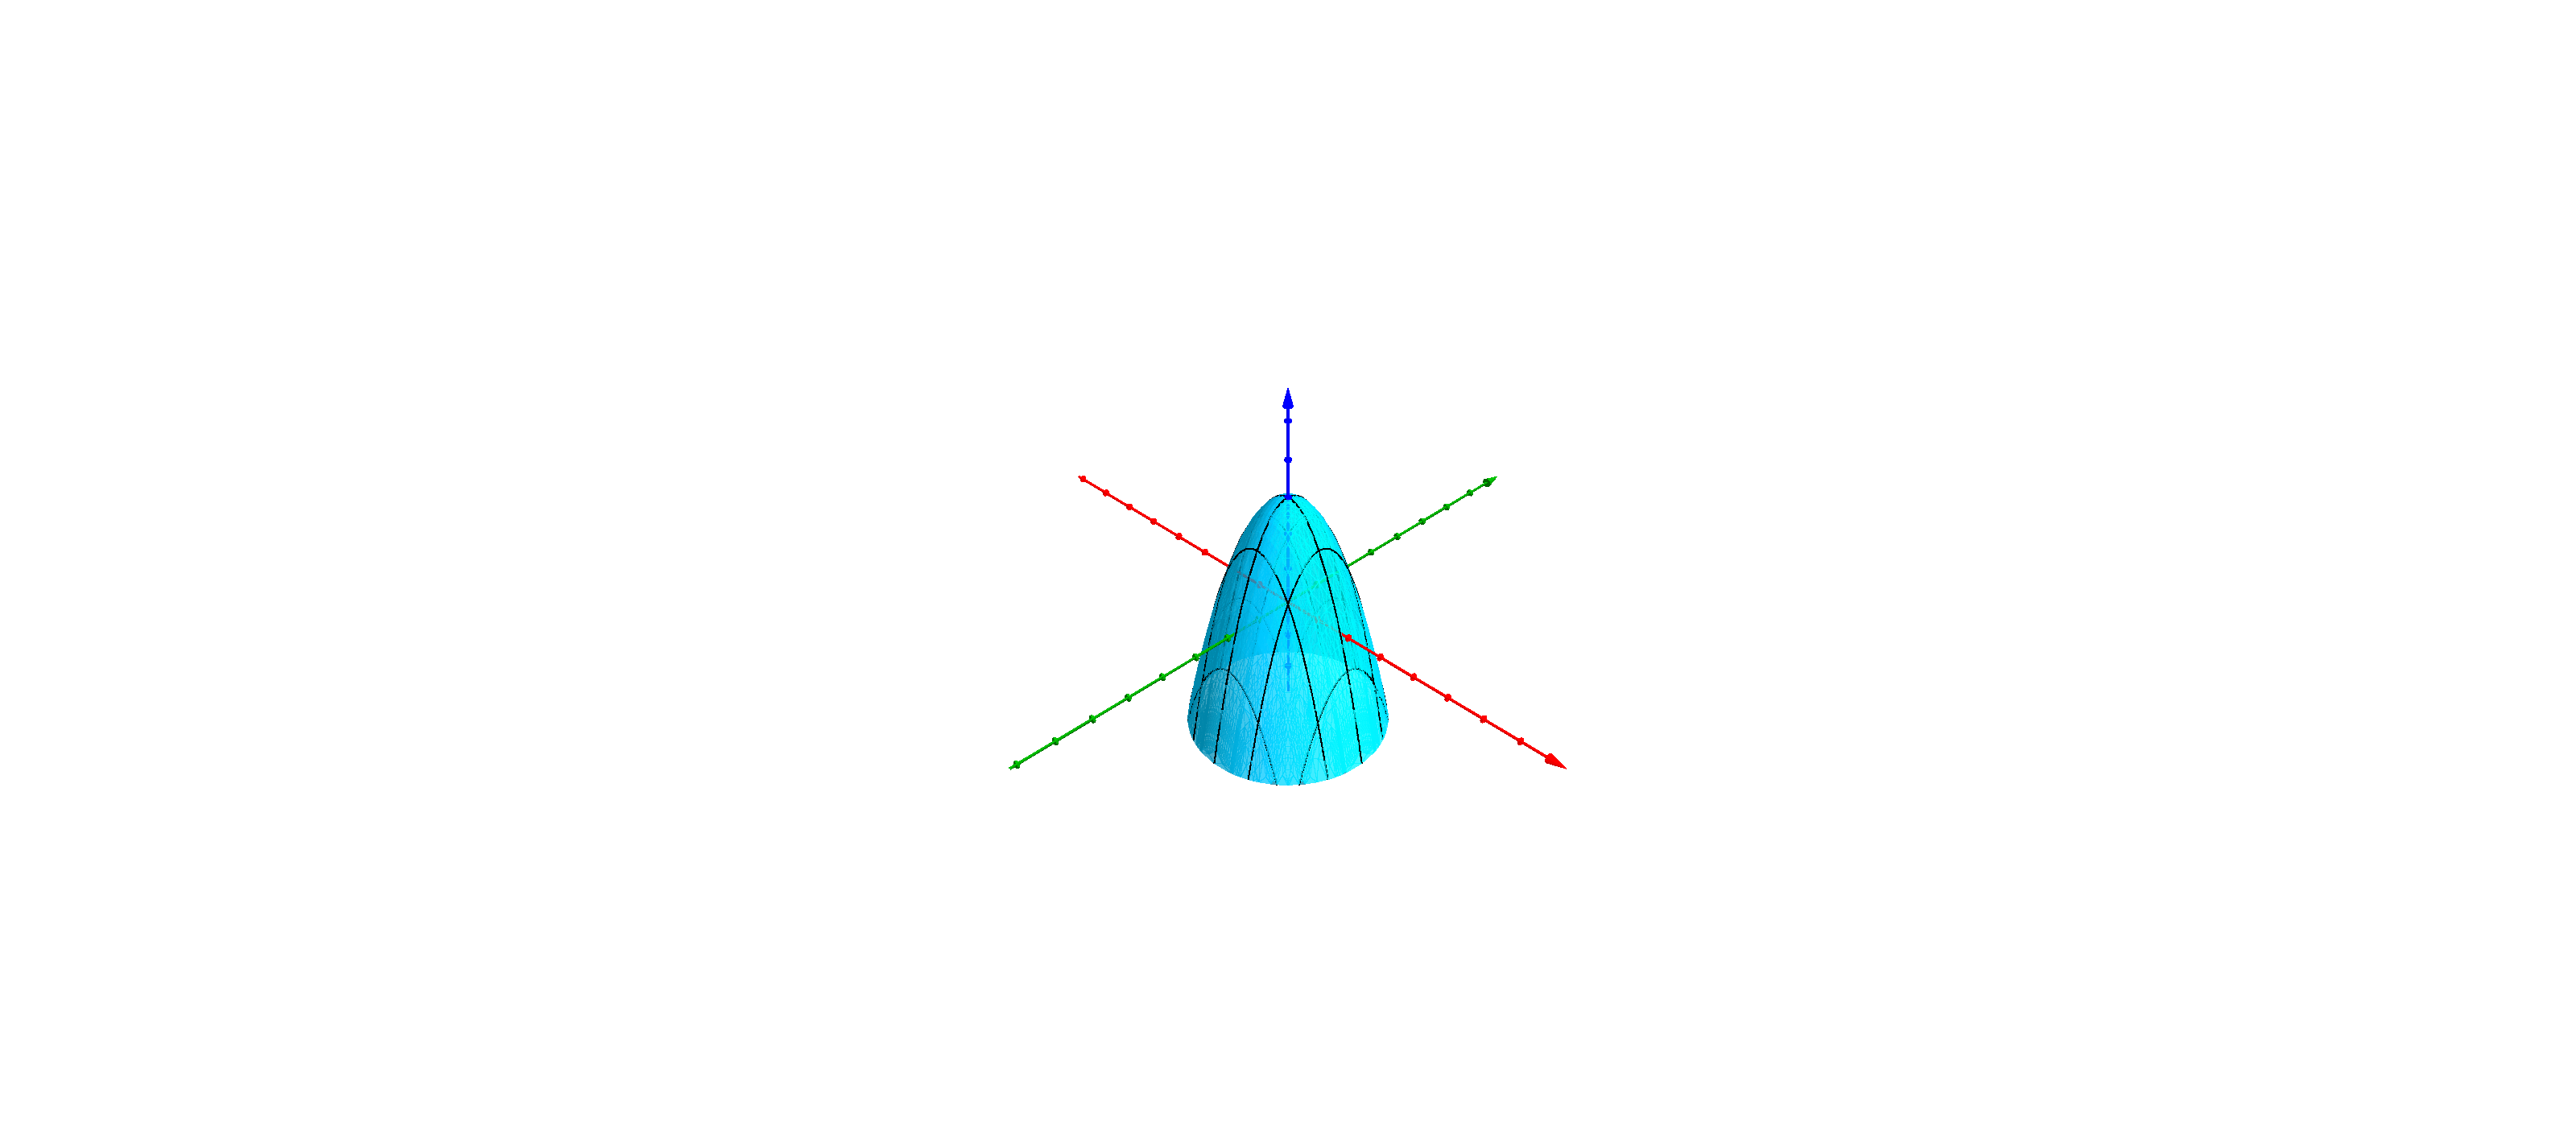
\includegraphics[width=0.7\linewidth]{paraboloid_reduced}	
		\label{fig:pd}
		\caption{พาราโบลอยด์ (พาราโบลาในปริภูมิ 3 มิติ)}
	\end{figure}

\section{สมการพาราโบลาปลอดภัย}
สมมติ เรายิงวัตถุจากจุดกำเนิดพิกัด (0,0) ด้วยอัตราเร็วต้น $u$ ไปในทิศทางและมุมใด ๆ ในสนามโน้มถ่วงที่มีค่า $g$\\

	\subsection{พิจารณาแกน $x$}
	เนื่องจากเป็นการเคลื่อนที่ ที่ไม่มีความเร่งจะได้ 
	$$\Delta x=u_xt$$
	สมมติยิงวัตถุทำมุม $\theta$ กับแนวระดับ
	$$x=u\cos\theta t$$
	\begin{equation}\label{x_eq}
	t=\frac{x}{u\cos\theta}
	\end{equation}
	
	\subsection{พิจารณาแกน $y$}
	เนื่องจากเป็นการเคลื่อนที่ ที่มีความเร่งจะได้
	$$\Delta y=u_yt+\frac{1}{2}a_yt^2$$
	สมมติยิงวัตถุทำมุม $\theta$ กับแนวระดับ
	\begin{equation}\label{y_eq}
	y=u\sin\theta t-\frac{1}{2}gt^2
	\end{equation}

	\subsection{พิจารณาแกน $x$ และแกน $y$}
	นำ (\ref{x_eq}) แทนใน (\ref{y_eq}) จะได้สมการบรรยายการเคลื่อนที่ ที่ไม่ขึ้นกับเวลา
	$$y=u\sin\theta (\frac{x}{u\cos\theta})-\frac{1}{2}g(\frac{x}{u\cos\theta})^2$$
	ทำการจัดรูป
	\begin{equation}\label{xy_eq}
	y=x\tan\theta-\frac{1}{2}\frac{gx^2}{u^2}\sec^2\theta
	\end{equation}
	จากเอกลักษณ์ตรีโกณมิติ
	$$\sec^2\theta-\tan^2\theta=1$$
	\begin{equation}\label{tri_id}
	\sec^2\theta=1+\tan^2\theta
	\end{equation}
	นำ (\ref{tri_id}) ไปแทนใน (\ref{xy_eq})
	$$y=x\tan\theta-\frac{1}{2}\frac{gx^2}{u^2}(1+\tan^2\theta)$$
	$$y=x\tan\theta-\frac{gx^2}{2u^2}-\frac{gx^2}{2u^2}\tan^2\theta$$
	$$0=\frac{gx^2}{2u^2}\tan^2\theta-x\tan\theta+(\frac{gx^2}{2u^2}+y)$$
	เราจะสังเกตได้ว่าสมการนี้เป็น Quadratic Equation ดังนั้นสามารถาค่า $\tan\theta$ ได้โดยใช้ Quadratic Formula
	$$\tan\theta = \dfrac{x\pm\sqrt{x^2-4\left(\dfrac{gx^2}{2u^2}\right)\left(\dfrac{gx^2}{2u^2}+y\right)}}{2\left(\dfrac{gx^2}{2u^2}\right)}$$
	$\tan\theta$ มีค่าจริง (จุด $(x,y)$ เป็นจุดที่สามารถยิงโพรเจกไทล์ไปได้) เมื่อภายในกรณฑ์ที่ 2\\ มีค่ามากกว่าเท่ากับ 0
	\begin{align*}
	x^2-4\left(\frac{gx^2}{2u^2}\right)\left(\frac{gx^2}{2u^2}+y\right)&\geqslant 0\\
	4\left(\frac{gx^2}{2u^2}\right)\left(\frac{gx^2}{2u^2}+y\right)&\leqslant x^2\\
	\frac{gx^2}{2u^2}+y&\leqslant \frac{u^2}{2g}\\
	y&\leqslant \frac{u^2}{2g}-\frac{gx^2}{2u^2}
	\end{align*}
	เนื่องจากเราต้องการสมการที่บอกขอบเขตของโพรเจกไทล์ที่สามารถเคลื่อนที่ไปได้ ดังนั้นสมการคือ
	\begin{equation}\label{pos}
	y= \frac{u^2}{2g}-\frac{gx^2}{2u^2}\quad\blacksquare
	\end{equation}
	\section{จุดที่น่าสนใจของพาราโบลาปลอดภัย}
	เนื่องจากสมการ (\ref{pos}) เป็นสามารพาราโบลา ดังนั้นสามารถจัดให้อยู่ในรูปมาตรฐานได้
	\begin{align*}
	y-\frac{u^2}{2g}&=-\frac{gx^2}{2u^2}\\
	-\frac{2u^2}{g}\left(y-\frac{u^2}{2g}\right)&=x^2
	\end{align*}
	\begin{equation}\label{pos_s}
	4\left(\frac{-u^2}{2g}\right)\left(y-\frac{u^2}{2g}\right)=x^2\quad\blacksquare
	\end{equation}
	เทียบได้กับสมการรูปมาตรฐานของพาราโบลา คือ
	$$4c(y-k)=(x-h)^2$$
\pagebreak
	วาดกราฟ (เฉพาะเส้นสีแดง) จะได้
	\begin{figure}[h]
		\centering
		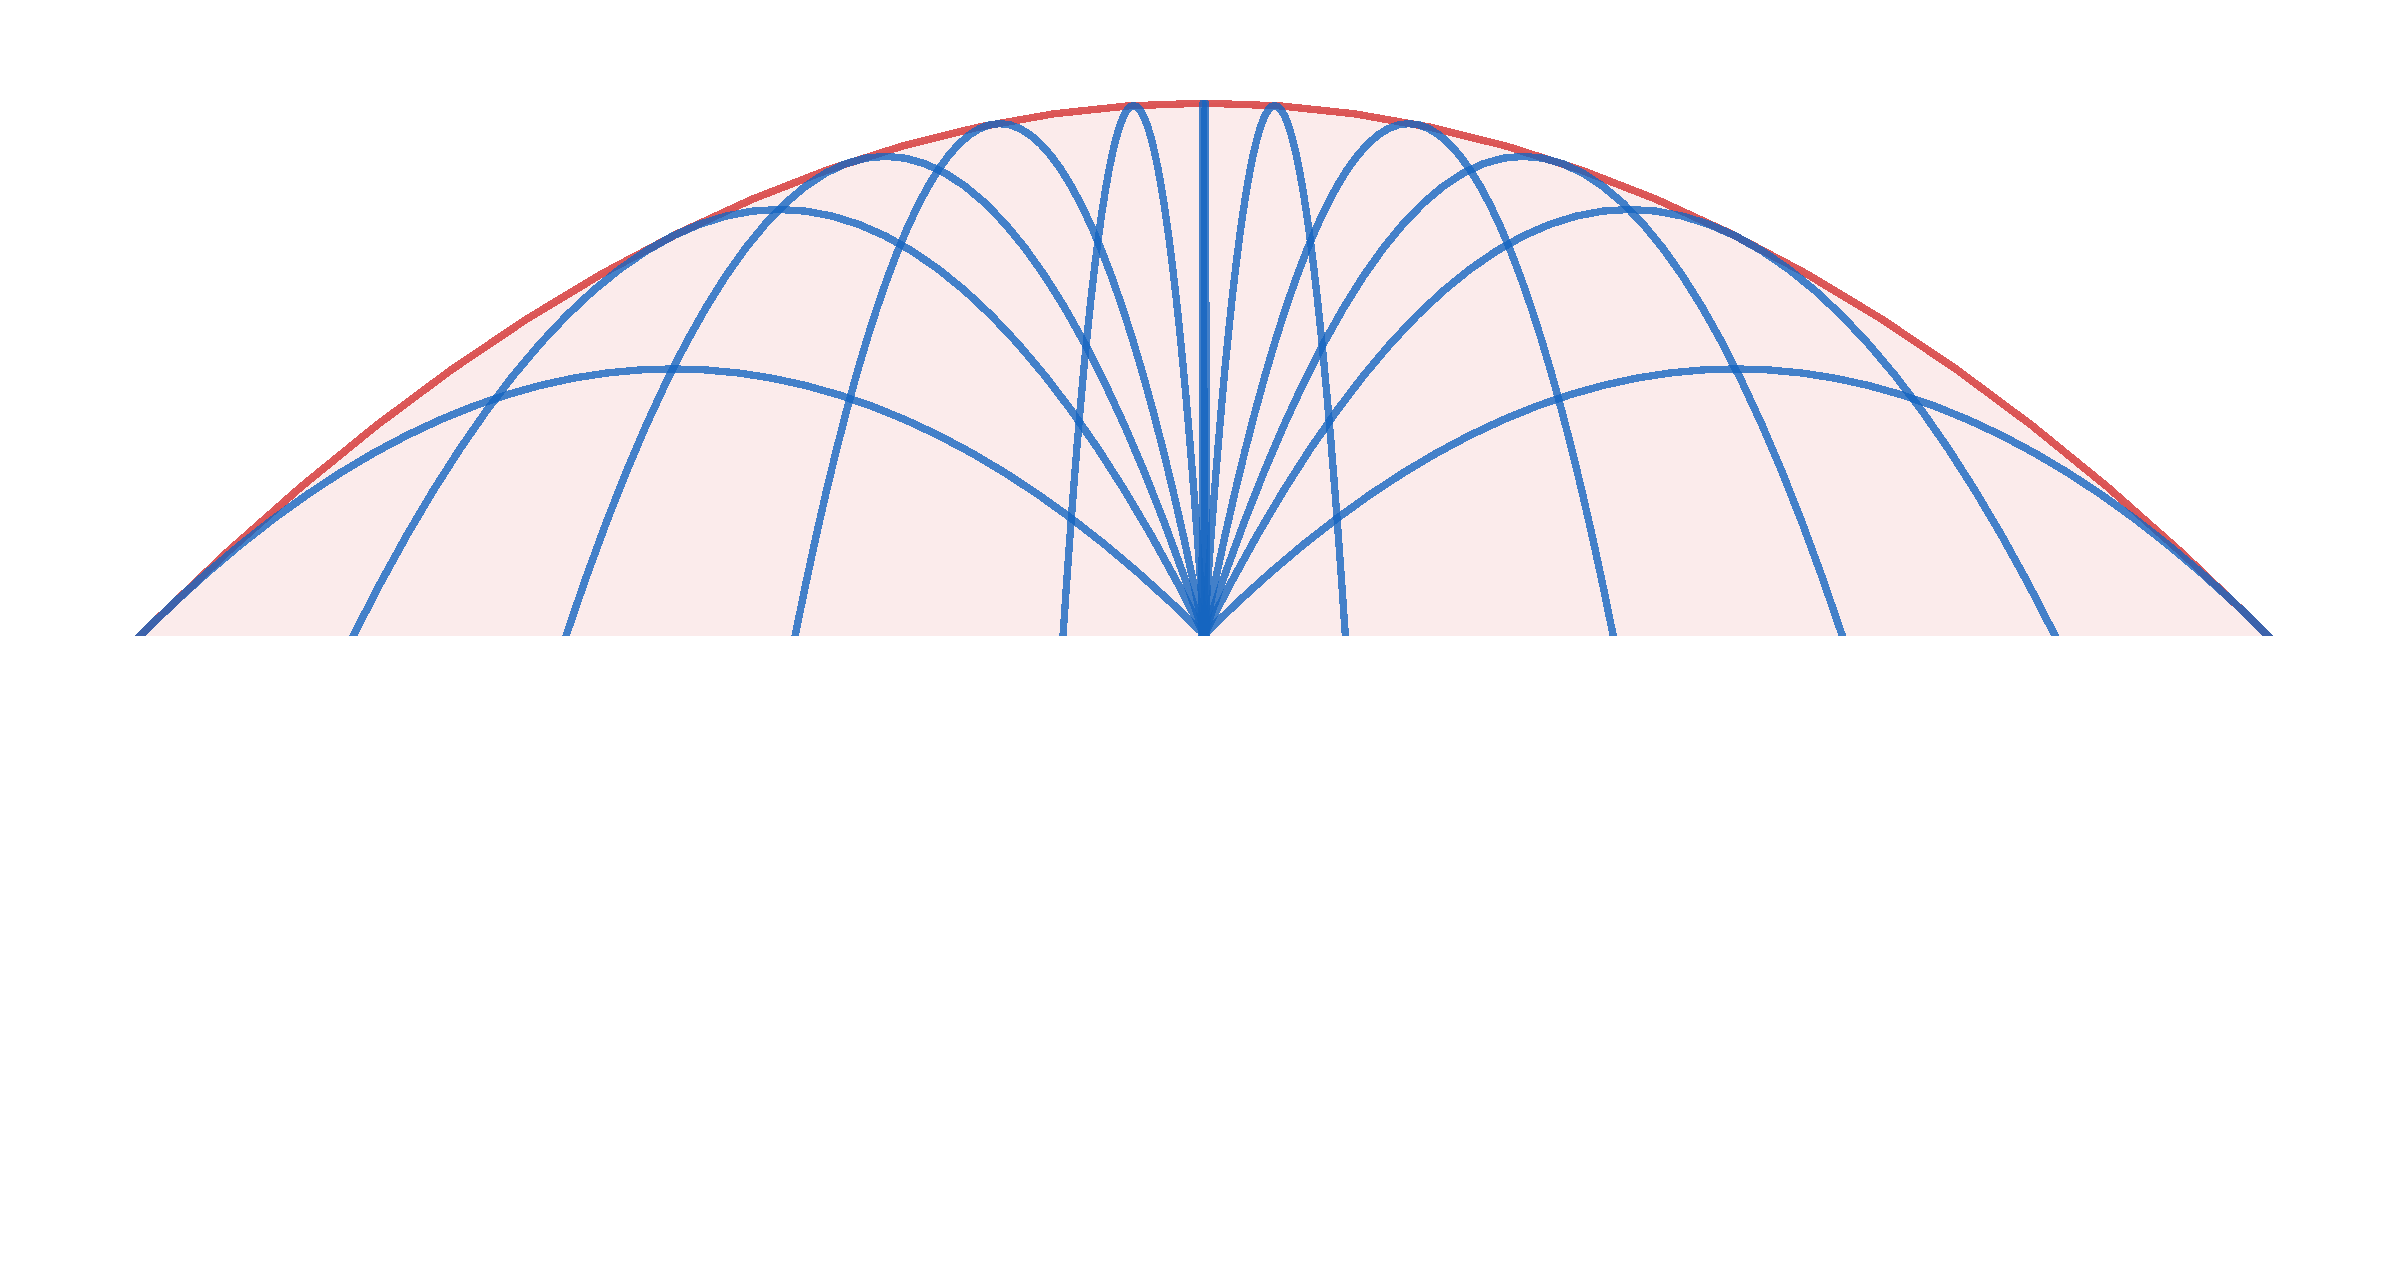
\includegraphics[width=1\linewidth]{pos_s3}	
		\label{fig:ps_s}
		\caption{พาราโบลาปลอดภัย (พื้นที่สีแดงคือบริเวณที่ยิงได้และสีน้ำเงินคือแนววิถีของโพรเจกไทล์)}
	\end{figure}
	\subsection{จุดยิง}
	เพราะพิจารณาการยิงวัตถุจากจุดกำเนิด (0,0) และพอคำนวณออกมาแล้วปรากฏว่าได้จุดโฟกัสของพาราโบลาปลอดภัยเป็นจุดกำเนิดเช่นกัน (พิจารณาจากสมการ (\ref{pos_s})) ดังนั้นสรุปได้ว่า \textbf{จุดยิงเป็นจุดโฟกัส}
	\subsection{ระยะสูงสุดในแนวดิ่ง}
	เนื่องจากจุดยิงเป็นจุดโฟกัส จะได้ว่าระยะจากจุดโฟกัสถึงจุดยอดเท่ากับ $\abs{c}=\dfrac{u^2}{2g}$ ก็คือการยิงวัตถุทำมุม $90\si{\degree}$ นั้นเอง
	\subsection{ระยะไกลสุดในแนวราบ}
	เนื่องจากจุดยิงเป็นจุดโฟกัส จะได้ Latus Rectum\footnote{ความกว้างของพาราโบลา}$=\abs{4c}=\dfrac{2u^2}{g}$ แต่เราต้องการแค่ครึ่งเดียวของ Latus Rectum (ระยะไกลสุดในแนวราบ) จะได้ $\dfrac{u^2}{g}$ ก็คือการยิงวัตถุทำมุม $45\si{\degree}$ นั้นเอง ซึึ่งค่านี้เราก็สามารถหาได้จากจุดตัดแกน $x$ ของกราฟพาราโบลาเช่นเดียวกัน
	\subsection{2 คำตอบ 2 มุม}
	เพราะว่าการแก้หา $\tan\theta$ เพื่อจะหาสมการพาราโบลาปลอดภัยเป็นการแก้ Quadratic Equation จะได้ 2 คำตอบเมื่อในค่าใต้กรณฑ์ที่ 2 มากกว่า 0 แสดงว่าจะมี 2 มุมที่สามารถยิงวัตถุไปที่จุด $(x,y)$ นั้นได้แต่ถ้าเท่ากับ 0 แสดงว่าจะมีเพียงมุมเดียวที่สามารถยิงไปได้ก็คือ จุดที่อยู่บนพาราโบลาปลอดภัยนั้นเอง
\section{ตัวอย่างการใช้งาน พาราโบลาปลอดภัย}
	สมมติ ยิงวัตถุด้วยอัตราเร็วต้น คือ 10 \si{m/s} และมีความเร่งเนื่องจากสนามโน้มถ่วง คือ 9.8 \si{m/s^2} จะวาดกราฟพาราโบลาปลอดภัยได้ดังนี้
	\begin{figure}[h]
	\centering
	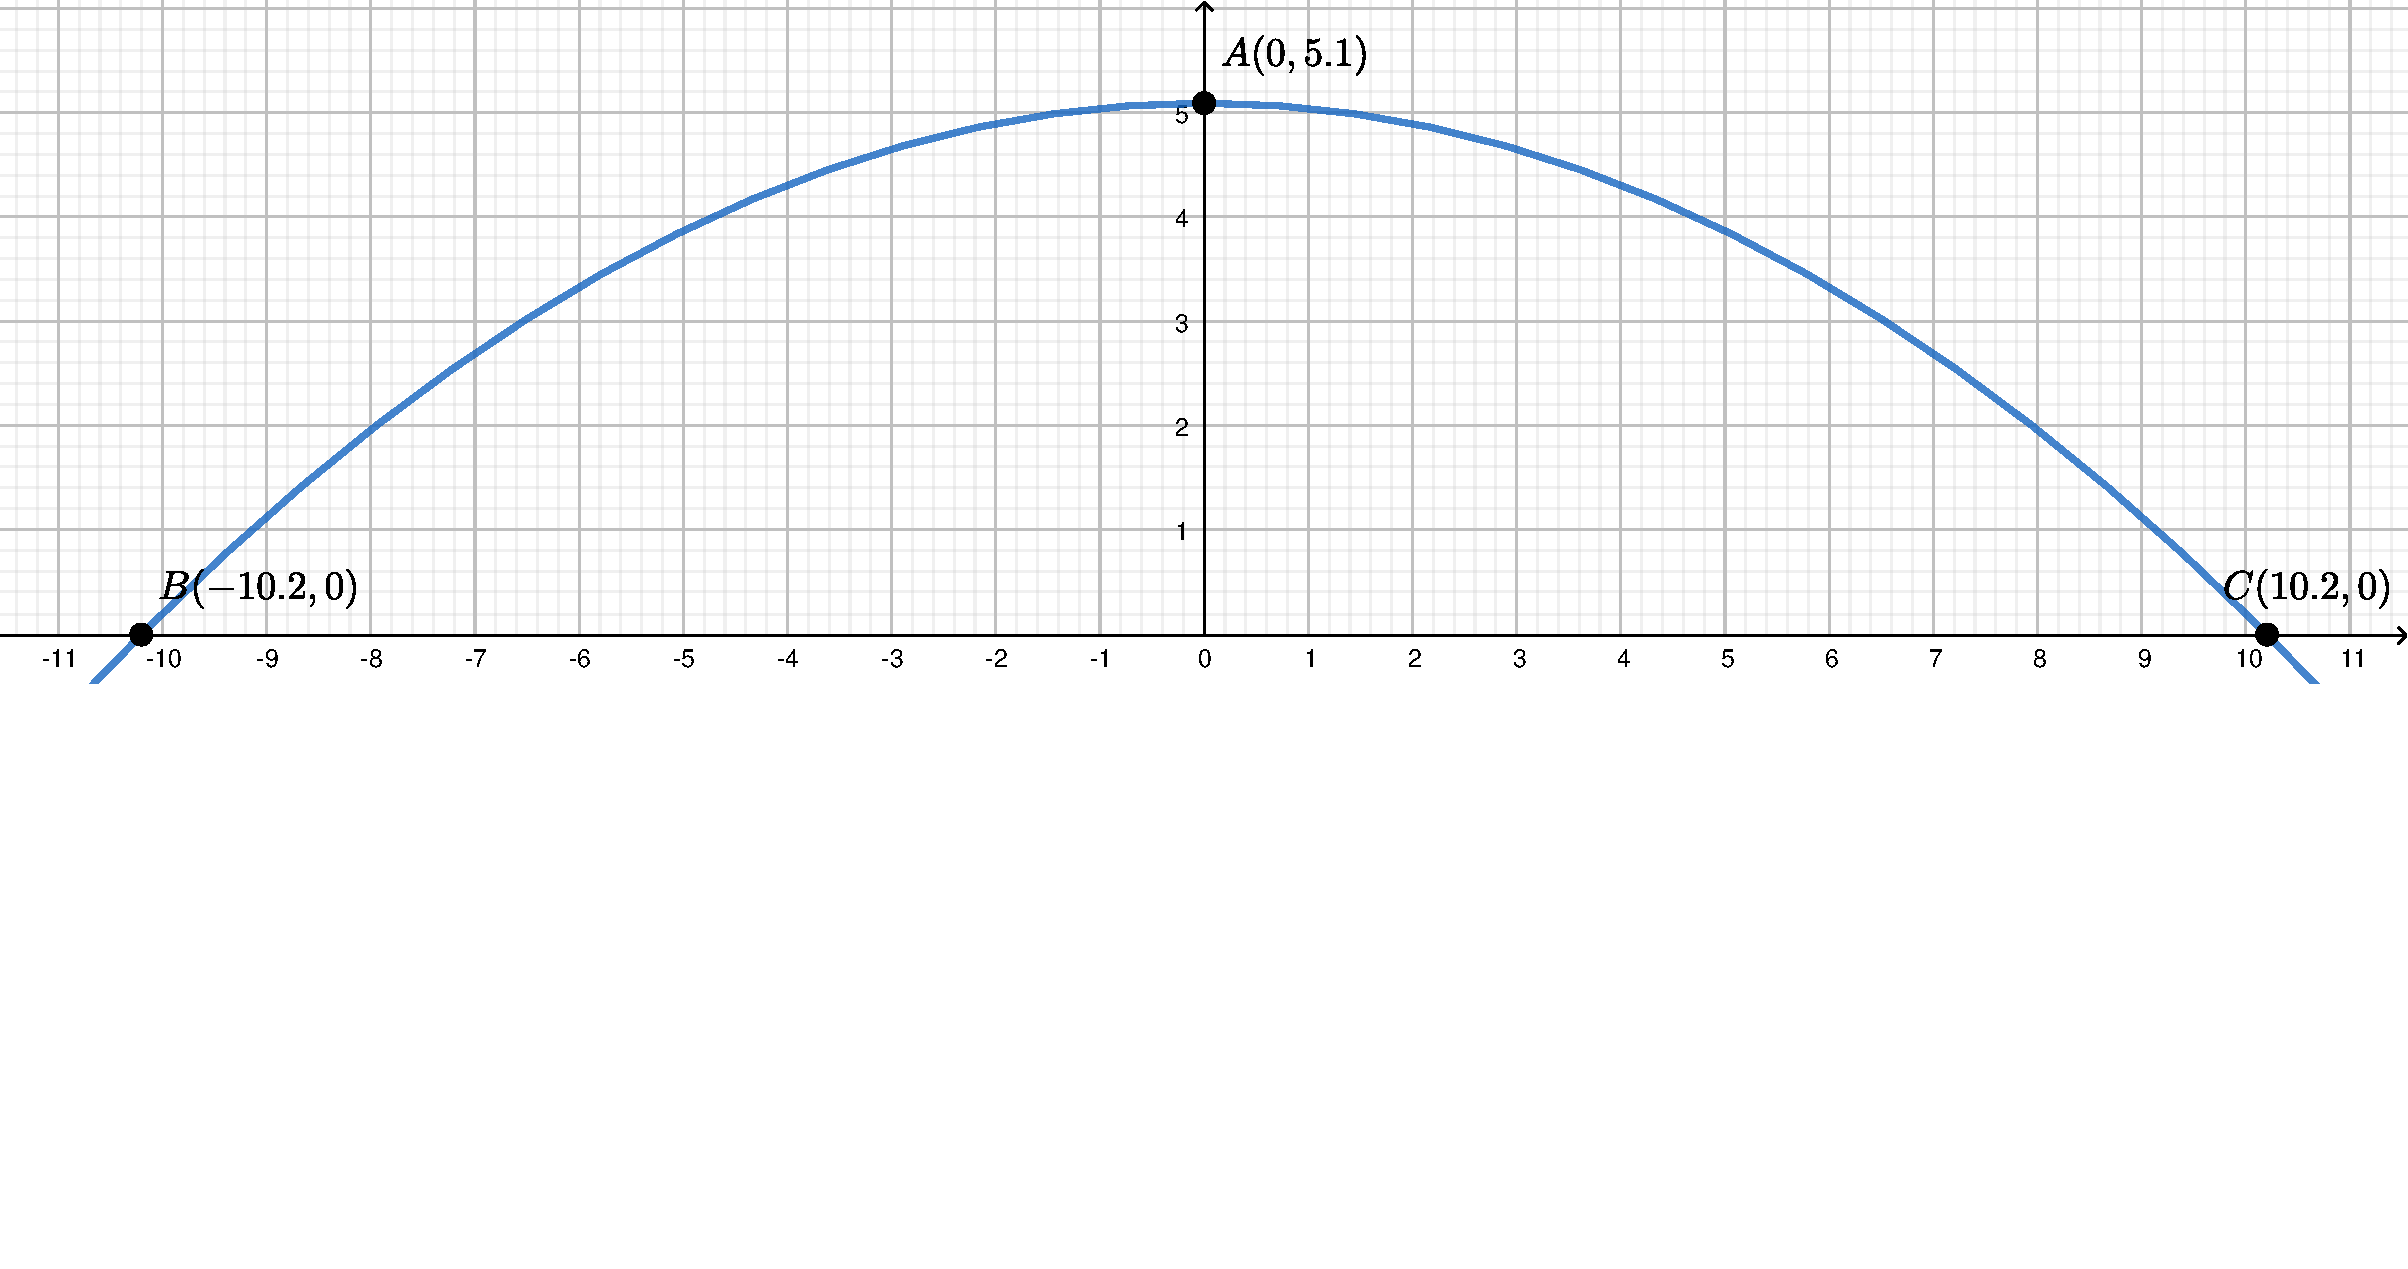
\includegraphics[width=1\linewidth]{pos}	
	\label{fig:pos}
	\end{figure}\\
	\\\indent ถ้าเราอยากรู้ว่า ถ้ายิงวัตถุจากจุด (0,0) โดยทำมุมกับแนวราบเท่าไรก็ได้แล้วจะได้ความสูงและระยะในแนวราบมากที่สุดเท่ากับเท่าไร\\
	ดูจากกราฟพาราโบลาปลอดภัยก็ตอบได้ทันทีเลยว่า ความสูงที่มากที่สุด $\approx 5.1\;\si{m}$ \\และระยะในแนวราบที่มากที่สุด $\approx 10.2\;\si{m}$\\
	\textbf{ถ้าไม่เชื่อก็ลองเช็กดูด้วยสูตรการเคลื่อนที่แนวตรงโดยมีความเร่งคงที่!}
\section{เว็บไซต์สำหรับอ่านเพิ่มเติม}
	\begin{enumerate}
		\item \url{https://bit.ly/3dlsqP9}
		\item \url{https://bit.ly/2SDfoEL}
		\item \url{http://mpec.sc.mahidol.ac.th/forums/index.php/topic,2343}
		\item \url{http://mpec.sc.mahidol.ac.th/forums/index.php/topic,345}
		\item \url{http://mpec.sc.mahidol.ac.th/forums/index.php/topic,2342}
	\end{enumerate}
\end{document}